%%% Local Variables: 
%%% mode: latex
%%% TeX-master: t
%%% End: 

\documentclass[a4paper,12pt]{article}

\usepackage{graphicx}
\usepackage{caption2}

\title{Using the {\tt MovingRegionAlgebra}}
\author{Holger M\"{u}nx {\tt $<$hm@muenx.net$>$}
    \thanks{The {\tt MovingRegionAlgebra} has been developed
    as bachelor thesis with Prof.\ Dr.\ Ralf Hartmut G\"{u}ting,
    Fernuniversit\"{a}t Hagen, Fachbereich Informatik, 
    Lehrgebiet Praktische Informatik IV}}
\date{22-Feb-2005 / INCOMPLETE DRAFT}

\newcommand{\secondo}{{\scshape SE\-CON\-DO}}
\newcommand{\mra}{{\tt Moving\-Region\-Algebra}}
\newcommand{\mr}{{\tt movingregion}}

\setlength{\parindent}{0em}
\setlength{\parskip}{1.5ex}

\renewcommand{\captionfont}{\bf}

\begin{document}

\maketitle

\begin{abstract}
This document provides a number of practical examples for the usage
of the \mra\ in the \secondo\ DBMS. It describes
both database objects, related queries and the application of
\secondo's Hoese viewer to display objects and query results.
\end{abstract}

\section{Introduction}

Spatial and temporal objects in databases are used to represent
real physical objects, which have a position and extension in space
as attributes, which can change over time. Examples of such objects
are countries, mountains and rivers or planes, cars and ships.
Pollution distribution or storm areas are examples for moving
regions. \cite{GuS04}, \cite{EGS+99}, \cite{GBE+00}, \cite{FGN+00}
and \cite{LFG03}
provide introductions to temporal objects on various levels.

\secondo\ is an extensible DBMS and is introduced in \cite{DiG99}.
Algebras can be added to \secondo\ to implement additional data types
and operators. The {\tt SpatialAlgebra}
and the \mra\ support spatial and selected temporal
objects. The \mra\ implements moving regions and
is described in \cite{Mue05}.

This document provides information about using the \mra. The
focus is on a very practical perspective, including numerous examples
and screenshots. Understanding the operator of \secondo and the moving
regions theory is required to apply this document. Please make sure that
the \mra\ is included in \secondo.

Section \ref{creating} explains methods to create
\mra\ objects. Section \ref{operations} describes operations on
\mra\ objects including different ways to visualise the results.

\section{Creating {\tt movingregion} objects}
\label{creating}

\subsection{Simple objects}

The following \secondo\ statement creates a simple \mr\ object {\tt mr1},
consisting
of a single region unit, which contains one face with a cycle and a hole
cycle. The unit's interval ranges from instant $0.0$ to instant $10.0$,
which are the
floating point representations of the instants {\tt 2000-01-03-00:00:00.000}
and {\tt 2000-01-03-00:00:00.000}.
\begin{verbatim}
let mr1 = 
  [ const movingregion value 
      (((0.0 10.0 TRUE TRUE)
        ((((1.0 3.5 1.5 1.5)
           (2.0 5.5 3.0 4.5)
           (3.0 6.5 3.5 5.0)
           (4.0 6.5 5.5 5.0)
           (4.0 5.5 5.5 4.5)
           (5.0 4.5 7.5 2.5)
           (5.0 2.5 7.5 1.0)
           (4.0 1.5 7.0 0.5)
           (3.0 1.5 2.5 0.5))
          ((2.0 3.0 3.0 2.0)
           (2.0 4.0 3.0 3.0)
           (3.0 4.0 4.0 3.0)
           (3.0 3.0 4.0 2.0)))))) ];
\end{verbatim}
Figure
\ref{creating:simple1} shows the object in the Hoese viewer in the initial
instant. A complete description of the list representation of \mr\ objects is
presented in \cite{LeB04}.
\begin{figure}
  \begin{center}
    \includegraphics[scale=0.4]{screenshot01.png}
  \end{center}
  \caption{A simple \mr\ object in the Hoese viewer}
  \label{creating:simple1}
\end{figure}

Region units may degenerate in two different ways:
\begin{itemize}
  \item Segments may be reduced
    to points in its initial or final instant (but not in both).
  \item A segment may be equal to other segments in
    the initial or final instant. A segment may be even equal to 
    segments in the initial and the final instant as long as it is not
    equal to the same segment in the initial and the final instant.
\end{itemize}
A region unit must not degenerate in other instants than its initial
or final instant. Section 4.3.3 in \cite{GuS04} and other literature
requires to use open
intervals for the degenerated instants; the current implementation of
the \mra\ is more flexible and treats degeneration properly.
Figure \ref{creating:simple2} contains examples of
degeneration in three region units.
\begin{figure}
  \begin{center}
    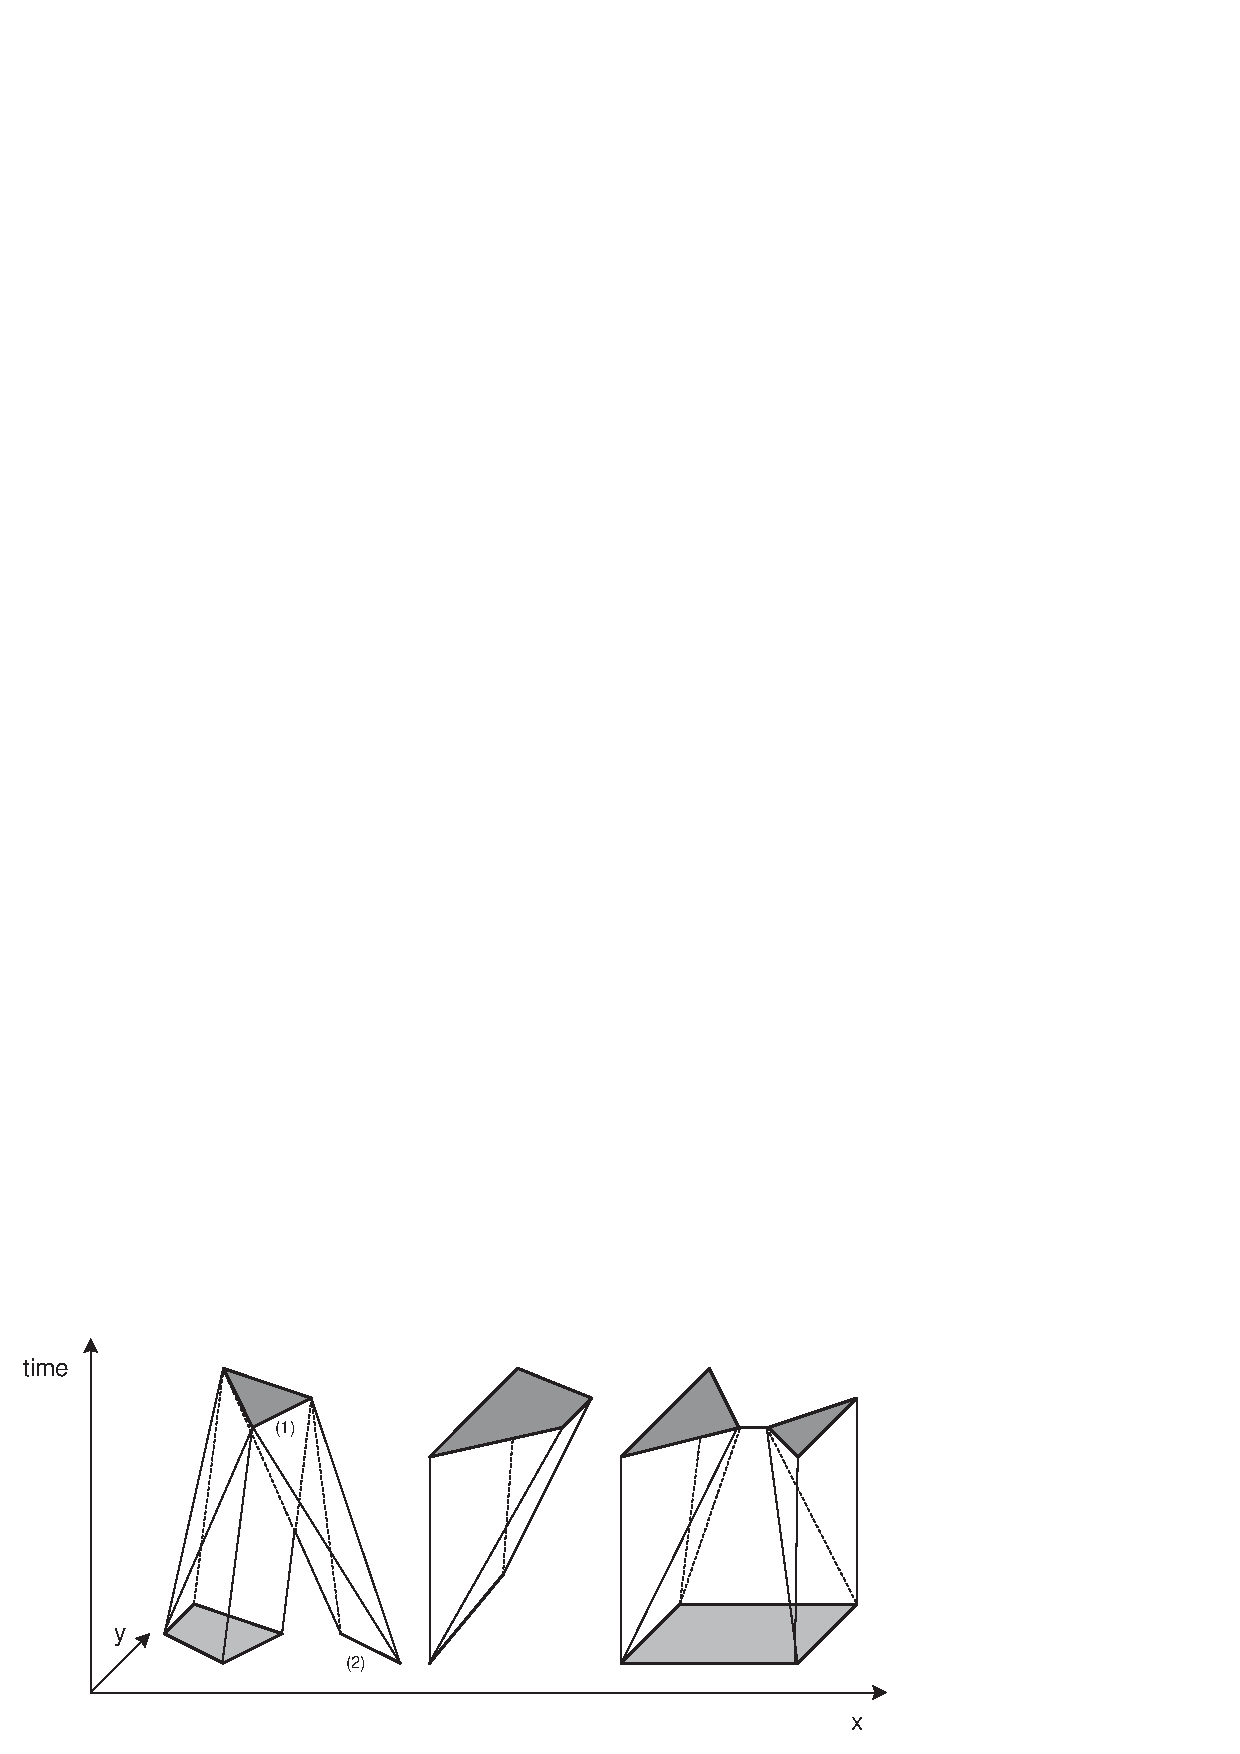
\includegraphics[scale=0.75]{uregion-degenerated.pdf}
  \end{center}
  \caption{Degenerated region units}
  \label{creating:simple2}
\end{figure}

The following statement creates a \mr\ object, whose single region
unit resembles the rightmost region unit in figure \ref{creating:simple2}.
\begin{verbatim}
let mr5 =
  [ const movingregion value
      (((0.0 10.0 TRUE TRUE)
        ((((2.0 1.0 1.0 4.0)
           (2.0 3.0 1.0 7.0)
           (2.0 3.0 3.0 6.0)
           (6.0 3.0 5.0 6.0)
           (6.0 3.0 7.0 6.0)
           (6.0 1.0 7.0 4.0)
           (6.0 1.0 5.0 6.0)
           (2.0 1.0 3.0 6.0)))))) ];
\end{verbatim}
In the initial instant, this object should be a region, which has the
shape of a rectangle. Lets apply the {\tt initial} operator to verify this.
\begin{verbatim}
Secondo => query initial(mr5);

No specific display function defined. Generic function used.
Type: intimeregion
Value: 
("2000-01-03" 
    (
        (
            (
                (6.0 1.0) 
                (2.0 1.0) 
                (2.0 3.0) 
                (6.0 3.0)))))
\end{verbatim}
This is exactly the expected result. Applying the {\tt final} operator
results in two faces, which have the shape of two triangles pointing to
each other, which is again exactly the expected result.
\begin{verbatim}
Secondo => query final(mr5);

No specific display function defined. Generic function used.
Type: intimeregion
Value:
("2000-01-13" 
    (
        (
            (
                (3.0 6.0) 
                (1.0 4.0) 
                (1.0 7.0))) 
        (
            (
                (7.0 4.0) 
                (5.0 6.0) 
                (7.0 6.0)))))
\end{verbatim}

Please note that segments, which degenerate to a point in the initial or
final instant, are a useful tool to bypass the algebra's requirement that
the segment must keep its orientation through the entire interval of its
unit. If you are facing situations where you cannot meet this requirement,
split the segment into two segments, where the first segment degenerates to
a point in the initial and the second segment degenerates to a point in the
final instant.

\subsection{The {\tt Region2MRegion} converter}

During development and initial tests with the \mra, it has been noticed
that there is not much suitable data available which can be used to build
\mr\ objects. As a workaround, Thomas Behr of the Feruniversit\"{a}t Hagen
has created the
{\tt Region2MRegion} converter, which applies a list of affine
transformations to a {\tt region} object to construct a \mr\ object.

Lets assume that the following {\tt region} objects exists in \secondo.
\begin{verbatim}
Secondo => query r1;

No specific display function defined. Generic function used.
Type: region
Value: 
(
    (
        (
            (136.0 47.0) 
            (91.0 25.0) 
            (59.0 45.0) 
            (42.0 82.0) 
            (60.0 114.0) 
            (40.0 138.0) 
            (60.0 168.0) 
            (99.0 157.0) 
            (142.0 167.0) 
            (164.0 136.0) 
            (126.0 88.0))))
\end{verbatim}
Use the {\em save} button in the Java GUI to save this object to a file
{\tt r1}.

The {\tt Region2MRegion} converter is located in the directory
\begin{verbatim}
  secondo/Tools/Converter/Region2MRegion
\end{verbatim}
Basic instruction can be found in the {\tt README} file.

Create a file {\tt r1.t} with the following contents.
\begin{verbatim}
(( (translate (100.0 0.0)) )
 ( (translate (100.0 100.0)) )
 ( (translate (100.0 0.0)) ))
\end{verbatim}
This instructs the {\tt Region2MRegion} to create a \mr\ object with
three region units. In the first unit, the region is moved 100 units
to the right. In the second unit, the region is moved 100 units up and
to the right. In the third unit, the region is moved 100 units to the
right again. Each unit has a fixed interval length of six hours and the first
unit's interval starts at {\tt 2000-01-03-00:00:00.000}; the converter does
not allow any other interval specification in the current version.
Lets apply the converter now and put the result into the
file {\tt r1.res}.
\begin{verbatim}
$ ./lintransform r1 r1.t r1.res
Building nested List from File r1 has taken 102 milliseconds
Building nested List from File r1.t has taken 21 milliseconds
processed 11 points
\end{verbatim}
Use the {\em load} button in the Java GUI to load this object. Loading
the file does not create an object in \secondo: Use the {\em store} button
to do this. You may need to rename the object with the {\em rename} button
before this is possible. Figure \ref{creating:r2mr1} shows the resulting
\mr\ object in a number of instants, where two hours are between each
shown instant. Please note the usage of the operators {\tt atinstant} and
{\tt val} to obtain the {\tt region} value of a \mr\ object in a specific
instant.
\begin{figure}
  \begin{center}
    \includegraphics[scale=0.4]{screenshot02.png}
  \end{center}
  \caption{A \mr\ object created with {\tt Region2MRegion}}
  \label{creating:r2mr1}
\end{figure}

\subsection{Object creation in the Hoese viewer}

\section{Operations on {\tt movingregion} Objects}
\label{operations}

\section{Other hints}

precision and rounding errors

\begin{thebibliography}{\hspace{2cm}}

\bibitem[DiG99]{DiG99}
  S.\ Dieker, R.\ H.\ G\"{u}ting.
  \textsl{Plug and Play with Query Algebras: \secondo\ A Generic DBMS
    Development Environment}.
  Informatik Berichte 249 - 2/1999, Fernuniversit\"{a}t Hagen, 1999.

\bibitem[EGS+99]{EGS+99}
  M.\ Erwig, R.\ H.\ G\"{u}ting, M.\ Schneider, M.\ Vazirgiannis.
  \textsl{Spatio-Temporal Data Types: An Approach to Modeling and
    Querying Moving Objects in Databases}.
  GeoInformatica 3:3, 1999.

\bibitem[FGN+00]{FGN+00}
  L.\ Forlizzi, R.\ H.\ G\"{u}ting, E.\ Nardelli, M.\ Schneider.
  \textsl{A Data Model and Data Structures for Moving Objects Databases}.
  Proceedings of the 2000 ACM SIGMOD International Conference on Management
  of Data, 2000.
  
\bibitem[GBE+00]{GBE+00}
  R.\ H.\ G\"{u}ting, M.\ H.\ B\"{o}hlen, M.\ Erwig, C.\ S.\ Jensen,
  N.\ A.\ Lorentzos, M.\ Schneider, M.\ Vazirgiannis.
  \textsl{A Foundation for Representing and Querying Moving Objects}.
  ACM Transactions on Database Systems, Vol. 25, No. 1, March 2000.

\bibitem[GuS04]{GuS04}
  R.\ H.\ G\"{u}ting, M.\ Schneider.
  \textsl{Moving Objects Databases}.
  Vorlesung an der Fernuniversit\"{a}t Hagen, 2004.

\bibitem[LeB04]{LeB04}
  J.\ A.\ C.\ Lema, T.\ Behr.
  \textsl{External Representation of Spatial and Spatio-Temporal Values}.

\bibitem[LFG03]{LFG03}
  J.\ A.\ C.\ Lema, L.\ Forlizzi, R.\ H.\ G\"{u}ting, E.\ Nardelli,
  M.\ Schneider.
  \textsl{Algorithms for Moving Objects Databases}.
  The Computer Journal, Vol. 46, No. 6, 2003.

\bibitem[Mue05]{Mue05}
  H.\ M\"{u}nx.
  \textsl{Behandlung zeitabh\"{a}ngiger Gebiete in Datenbanken
    f\"{u}r bewegte Objekte}.
  Bachelor thesis, Fernuniversit\"{a}t Hagen, 2005.

\end{thebibliography}

\end{document}
